\begin{question}
\noindent Triangle $T$ is enlarged to give triangle $T'$, as shown on the grid below.

\begin{center}
\scalebox{0.75}{
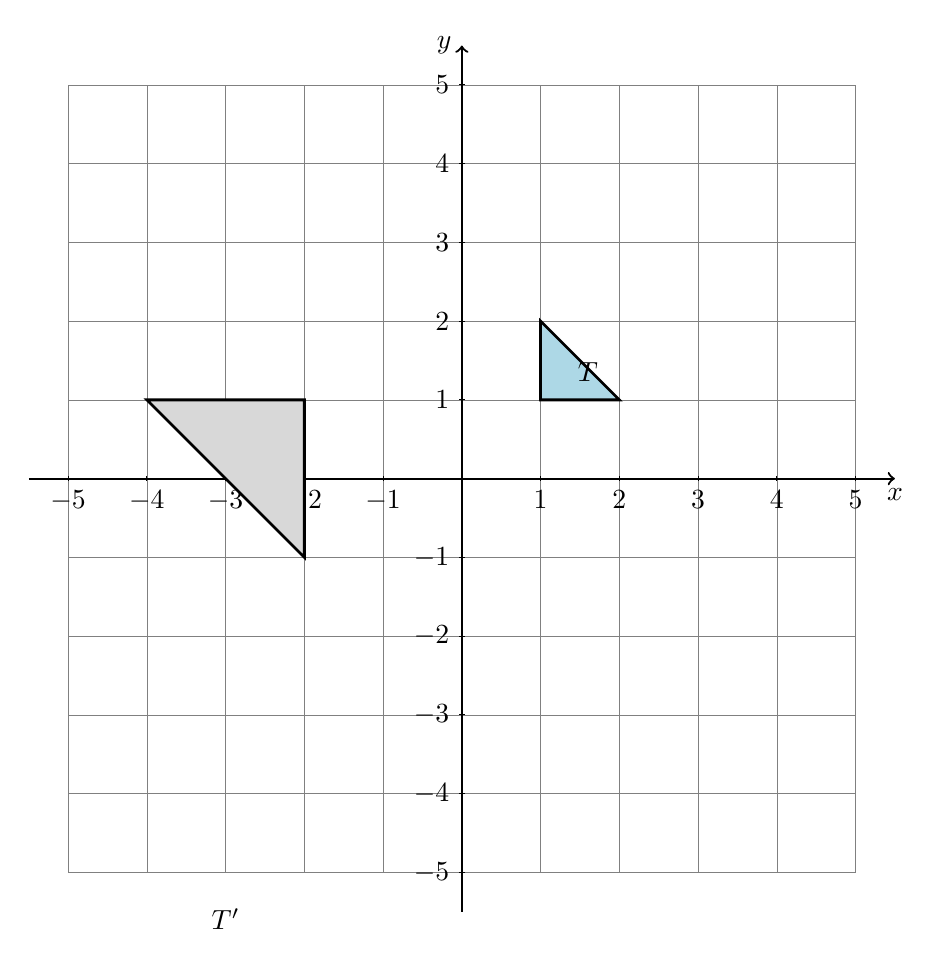
\begin{tikzpicture}
    \definecolor{borderColour}{HTML}{000000}
    \definecolor{fillColourT}{HTML}{ADD8E6}
    \definecolor{fillColourTprime}{HTML}{D8D8D8}

    \def\axisLimit{5}

    % Draw grid
    \draw[step=1cm,gray,very thin] (-\axisLimit,-\axisLimit) grid (\axisLimit,\axisLimit);

    % Draw axes
    \draw[thick,->] (-\axisLimit-0.5,0) -- (\axisLimit+0.5,0) node[anchor=north] {$x$};
    \draw[thick,->] (0,-\axisLimit-0.5) -- (0,\axisLimit+0.5) node[anchor=east] {$y$};

    % Label x-axis and y-axis
    \foreach \x in {-\axisLimit,...,-1,1,2,...,\axisLimit}
        \draw (\x cm,1pt) -- (\x cm,-1pt) node[anchor=north] {$\x$};
    \foreach \y in {-\axisLimit,...,-1,1,2,...,\axisLimit}
        \draw (1pt,\y cm) -- (-1pt,\y cm) node[anchor=east] {$\y$};

    % Define vertices of T
    \coordinate (A) at (1,1);
    \coordinate (B) at (1,2);
    \coordinate (C) at (2,1);

    % Draw T
    \draw[fill=fillColourT, draw=borderColour, line width=1pt] (A) -- (B) -- (C) -- cycle;
    \node at (1.6,1.35) {$T$};

    % Define vertices of T' (enlargement by scale factor -2 from centre (0,-1))
    \coordinate (centre) at (0,1);
    \coordinate (Ap) at ([scale around={-2:(centre)}]A);
    \coordinate (Bp) at ([scale around={-2:(centre)}]B);
    \coordinate (Cp) at ([scale around={-2:(centre)}]C);

    % Draw T'
    \draw[fill=fillColourTprime, draw=borderColour, line width=1pt] (Ap) -- (Bp) -- (Cp) -- cycle;
    \node at (-3,-5.6) {$T'$};

\end{tikzpicture}
}
\end{center}

\noindent Find the scale factor of the enlargement and the coordinates of the centre of enlargement.

\vspace{5cm}

\begin{flushright}
    \answerplain{3}
\end{flushright}
\end{question}
